%\documentclass{standalone}
%\usepackage{graphicx}
%\usepackage[usenames,dvipsnames,svgnames,table]{xcolor}
%\usepackage{tikz,ulem}
%\begin{document}

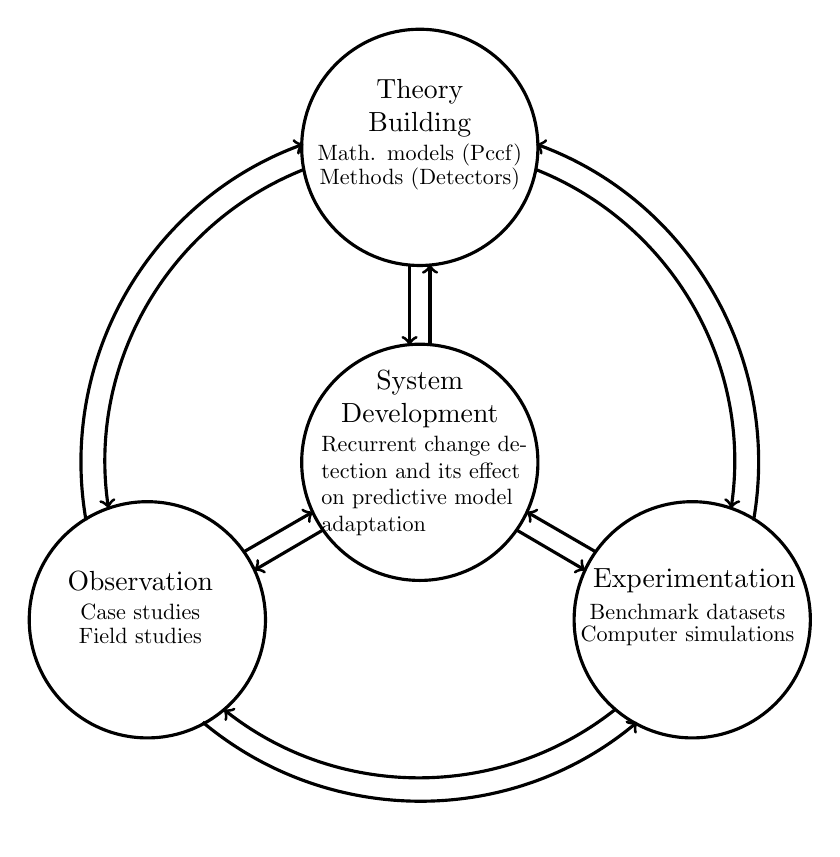
\begin{tikzpicture}[scale = 1]

% START: Rust generated
  \draw [black, line width=0.4mm] (0.00, 0.00) circle [radius=1.5];
  \draw [black, line width=0.4mm] (0.00, 4.00) circle [radius=1.5];
  \draw [black, line width=0.4mm] (3.46, -2.00) circle [radius=1.5];
  \draw [black, line width=0.4mm] (-3.46, -2.00) circle [radius=1.5];
  \draw [->, line width=0.4mm] (1.23, -0.86) -- (2.10, -1.37);
  \draw [->, line width=0.4mm] (2.24, -1.14) -- (1.36, -0.63);
  \draw [->, line width=0.4mm] (-1.23, -0.86) -- (-2.10, -1.37);
  \draw [->, line width=0.4mm] (-2.24, -1.14) -- (-1.36, -0.63);
  \draw [->, line width=0.4mm] (0.13, 1.49) -- (0.13, 2.51);
  \draw [->, line width=0.4mm] (-0.13, 2.51) -- (-0.13, 1.49);
  \draw[->, line width=0.4mm] (-1.47,3.72) arc [radius=4.00, start angle = 111.61, end angle = 188.39];
  \draw[->, line width=0.4mm] (1.47,3.72) arc [radius=4.00, start angle = 68.39, end angle = -8.39];
  \draw[->, line width=0.4mm] (2.48,-3.14) arc [radius=4.00, start angle = 308.39, end angle = 231.61];
  \draw[<-, line width=0.4mm] (-1.48,4.04) arc [radius=4.30, start angle = 110.09, end angle = 189.91];
  \draw[<-, line width=0.4mm] (1.48,4.04) arc [radius=4.30, start angle = 69.91, end angle = -9.91];
  \draw[<-, line width=0.4mm] (2.76,-3.30) arc [radius=4.30, start angle = 309.91, end angle = 230.09];

% END: Rust generated
  \node[text width=2cm, align=center] at (0, 0.8) {System \uline{Development}};
  \node[text width=3.5cm, scale=0.8] at (0.15, -0.3) {Recurrent change detection and its effect on predictive model adaptation};

  \node[text width=2cm, align=center]  at (0,4.5) {Theory \uline{Building}};
  \node[text width=5cm,align=center, scale=0.8] at (0, 3.9) {Math. models (Pccf)};
  \node[text width=5cm,align=center, scale=0.8] at (0, 3.6) {Methods (Detectors)};

  \node[text width=2cm, align=center]  at (-3.55, -1.5) {\uline{Observation}};
  \node[align=center,scale=0.8]  at (-3.55, -1.9) {Case studies};
  \node[align=center,scale=0.8]  at (-3.55, -2.2) {Field studies};

  \node[text width=2cm, align=center]  at (3.2, -1.5) {\uline{Experimentation}};
  \node[align=center,scale=0.8]  at (3.4, -1.9) {Benchmark datasets};
  \node[align=center,scale=0.8]  at (3.4, -2.2) {Computer simulations};

\end{tikzpicture}

%\end{document}
